% Dit werk is gelicenseerd onder de licentie Creative Commons Naamsvermelding-GelijkDelen 4.0 Internationaal. Ga naar http://creativecommons.org/licenses/by-sa/4.0/ om een kopie van de licentie te kunnen lezen.
\documentclass[t]{beamer}

% vaak gebruikte packages, nederlands
\usepackage[margin=2.5cm]{geometry}     % Marges instellen
\usepackage[dutch]{babel}               % Voor nederlandstalige hyphenatie (woordsplitsing)
\usepackage{amsmath,amsthm}             % Uitgebreide wiskundige mogelijkheden
\usepackage{url}                        % Om url's te verwerken
\usepackage{graphicx,subfigure}         % Om figuren te kunnen verwerken
\usepackage{color}
\usepackage{framed}
\usepackage{multicol}
\usepackage[small,bf,hang]{caption}     % Om de captions wat te verbeteren
\usepackage[utf8]{inputenc}             % Om niet ascii karakters rechtstreeks te kunnen typen
\usepackage{float}                      % Om nieuwe float environments aan te maken. Ook optie H!
\usepackage{flafter}                    % Opdat floats niet zouden voorsteken
\usepackage[section]{placeins}			% Om ervoor te zorgen dat floats binnen dezelfde section blijven
\usepackage[nottoc]{tocbibind}			% Bibliografie en inhoudsopgave in ToC; zie tocbibind.dvi
\usepackage{fancyhdr}                   % Voor fancy headers en footers
\usepackage{thmtools}                   % theorem tools
\usepackage{parskip}                    % Om paragrafen met een verticale spatie ipv horizontaal te laten beginnen
\usepackage[plainpages=false]{hyperref} % Om hyperlinks te hebben in het pdfdocument.



%%%%%%%%%%%%%%%%%%%%%%%%%%%%%%
% Algemene instellingen van het document.
%%%%%%%%%%%%%%%%%%%%%%%%%%%%%%
\renewcommand{\baselinestretch}{1.2} 	% De interlinie afstand wat vergroten.
\setcounter{MaxMatrixCols}{50}          % Max 20 kolommen in een matrix


%%%%%%%%%%%%%%%%%%%%%%%%%%%%%%
% Headers en footers
%%%%%%%%%%%%%%%%%%%%%%%%%%%%%%
\pagestyle{fancy}
\fancyhf{}
\renewcommand{\headrulewidth}{0pt}
\fancyhead[RO] {\rightmark}
\fancyhead[LE] {\leftmark}
\fancyfoot[RO,LE] {\thepage}

% no dot after chapter number
\renewcommand{\chaptermark}[1]{
	\markboth{\MakeUppercase{ \chaptername\ \thechapter\quad #1}}{}
}
% no dot after section number
\renewcommand{\sectionmark}[1]{
	\markright{\MakeUppercase{ \thesection\quad #1}}{}
}

% page header and footer style in mainmatter aanpassen
\let\newmainmatter\mainmatter
\renewcommand{\mainmatter}{

	\pagestyle{fancy}
	\fancyhf{}
	\renewcommand{\headrulewidth}{0pt}
	\fancyhead[RO] {\rightmark}
	\fancyhead[LE] {\leftmark}
	\fancyfoot[RO,LE] {\thepage}
	\fancyfoot[C]{\tiny{Brecht Baeten}}

	\newmainmatter
}
\let\newappendix\appendix
\renewcommand{\appendix}{
	\fancyfoot{}
	\fancyfoot[RO,LE] {\thepage}
	\newappendix
}


%%%%%%%%%%%%%%%%%%%%%%%%%%%%%%
% Nieuwe omgevingen
%%%%%%%%%%%%%%%%%%%%%%%%%%%%%%
\definecolor{shadecolor}{gray}{0.95}
\newcounter{voorbeeldcounter}[chapter]
\renewcommand{\thevoorbeeldcounter}{\thechapter.\arabic{voorbeeldcounter}}
\makeatletter
\newenvironment{voorbeeld}
{
\vspace{3mm}
\addtolength{\leftskip}{5mm}
\begin{shaded*}
\vspace{-3mm}
\refstepcounter{voorbeeldcounter}
\noindent
\textbf{Voorbeeld \thevoorbeeldcounter:\\}
%\vspace{-8mm}
%\begin{multicols}{2}
}
{
%\end{multicols}
\end{shaded*}
\addtolength{\leftskip}{-5mm}
}
\makeatother  
    
%%%%%%%%%%%%%%%%%%%%%%%%%%%%%%
% .svg commando's
%%%%%%%%%%%%%%%%%%%%%%%%%%%%%%
% nieuw commando om svg files dynamisch te updaten
%\newcommand{\executeiffilenewer}[3]{%
%\ifnum\pdfstrcmp{\pdffilemoddate{#1}}%
%{\pdffilemoddate{#2}}>0%
%{\immediate\write18{#3}}\fi%
%}
%% nieuw commando om. svg figuren in te voegen
%% Gebruik: \includesvg{path/filename.svg}
%\newcommand{\includesvg}[2][0]{%
%\executeiffilenewer{#2.svg}{#2.pdf}%
%{inkscape -z -C --file=#2.svg %
%--export-pdf=#2.pdf --export-latex}%
%\ifx#10
%	\let\svgwidth\undefined
%\else
%	\def\svgwidth{#1}
%\fi%
%\input{#2.pdf_tex}%
%\ifx \svgwidth\undefined
%\else
%	\let\svgwidth\undefined
%\fi%
%}

% nieuw commando om .fig figuren in te voegen
\newcommand{\includefig}[2][0]{%
\ifx#10
	\let\figwidth\undefined
\else
	\def\figwidth{#1}
\fi%
\input{#2.pdf_tex}%
\ifx \figwidth\undefined
\else
	\let\figwidth\undefined
\fi%
}

%%%%%%%%%%%%%%%%%%%%%%%%%%%%%%
% Packages
%%%%%%%%%%%%%%%%%%%%%%%%%%%%%%

%\usepackage{geometry}              	% 
\usepackage[dutch]{babel}               % Voor nederlandstalige hyphenatie (woordsplitsing)
\uselanguage{dutch}
\languagepath{dutch}
\usepackage{amsmath,amsthm}             % Uitgebreide wiskundige mogelijkheden
\usepackage{url}                        % Om url's te verwerken
\usepackage{graphicx,subfigure}         % Om figuren te kunnen verwerken
\usepackage[utf8]{inputenc}             % Om niet ascii karakters rechtstreeks te kunnen typen
\usepackage[section]{placeins}			% Om ervoor te zorgen dat floats binnen dezelfde section blijven
\usepackage{multicol}
\usepackage[absolute,overlay]{textpos}

%%%%%%%%%%%%%%%%%%%%%%%%%%%%%%
% Layout
%%%%%%%%%%%%%%%%%%%%%%%%%%%%%%
\usetheme{Frankfurt}
\usefonttheme[onlymath]{serif}
\AtBeginSection[]
{
  \begin{frame}
    \frametitle{Inhoud}
    \tableofcontents[currentsection]
  \end{frame}
}

\setbeamertemplate{navigation symbols}{}
\setbeamertemplate{footline}[page number]

%%%%%%%%%%%%%%%%%%%%%%%%%%%%%%
% Title
%%%%%%%%%%%%%%%%%%%%%%%%%%%%%%
\title{Fluïdummechanica}
\author{Brecht Baeten\inst{1}}
\institute{
	\inst{1}%
  		KU Leuven, Technologie campus Diepenbeek,\\ e-mail: brecht.baeten@kuleuven.be
}
\date{\today}
%%%%%%%%%%%%%%%%%%%%%%%%%%%%%%
% Omgevingen
%%%%%%%%%%%%%%%%%%%%%%%%%%%%%%


\subtitle{Controlevolumes}

\begin{document}

	\frame{\titlepage}
	\section{Inleiding}
	\begin{frame}
		\frametitle{Voorbeeld}
		\center
    		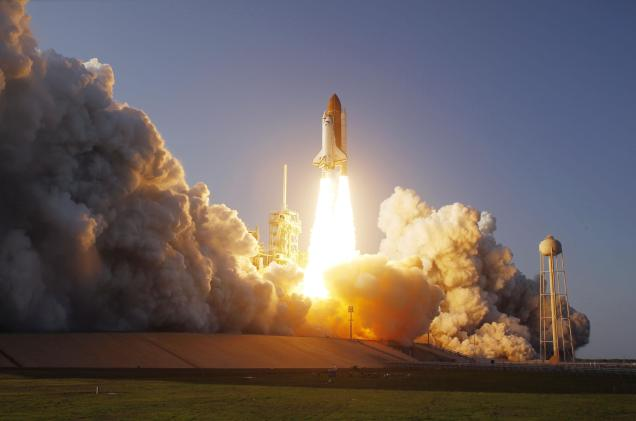
\includegraphics[height=0.8\textheight]{fig/controlevolumes/space_shuttle.jpg}\\
		\footnotesize{Bron: http://www.nasa.gov/}
  	\end{frame}
%%%%%%%%%%%%%%%%%%%%%%%%%%%%%%%%%%%%%%%%%%%%%%%%%%%%%%%%%%%%%%%%%%%%%%%%%%%
  	\section{Controle massa's}	
  	\begin{frame}
		\frametitle{Mechanica en Thermodynamica}
		\vspace{1cm}
		\pause 
		Behoud van massa
		\begin{equation}
			\frac{\diff m}{\diff t} = 0
		\end{equation}
		
		\pause 			
		Behoud van impuls
		\begin{equation}
			\frac{\diff \vt{P}}{\diff t} = \vt{F}
		\end{equation}
		
		\pause 
		Behoud van energie
		\begin{equation}
			\frac{\diff E}{\diff t} = \dot{Q}-\dot{W}
		\end{equation}
  	\end{frame}
%%%%%%%%%%%%%%%%%%%%%%%%%%%%%%%%%%%%%%%%%%%%%%%%%%%%%%%%%%%%%%%%%%%%%%%%%%%
  	\section{Controlevolumes}	
  	\begin{frame}
		\frametitle{Controlevolume}
		\center
		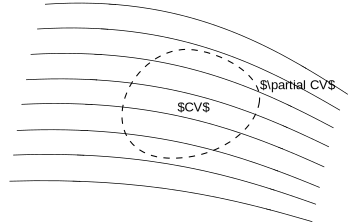
\includegraphics{fig/controlevolumes/Controlevolume_met_stroomlijnen}
  	\end{frame}
%%%%%%%%%%%%%%%%%%%%%%%%%%%%%%%%%%%%%%%%%%%%%%%%%%%%%%%%%%%%%%%%%%%%%%%%%%%
  	\begin{frame}
		\frametitle{Behoud van massa}
		\vspace{1cm}
		\begin{equation*}
			\left[
				\begin{array}{c}
					\mbox{De verandering} \\ \mbox{van massa in} \\ \mbox{het controlevolume}
				\end{array}
			\right]
			+
			\left[
				\begin{array}{c}
					\mbox{De netto} \\ \mbox{massastroom uit} \\ \mbox{het controlevolume}
				\end{array}
			\right]
			= 0
		\end{equation*}
		\vspace{1cm}
		\pause
		\begin{equation*}
			\frac{\diff m_{CV}}{\diff t} + \dot{m}_{\partial CV} = 0
		\end{equation*}
	\end{frame}	
%%%%%%%%%%%%%%%%%%%%%%%%%%%%%%%%%%%%%%%%%%%%%%%%%%%%%%%%%%%%%%%%%%%%%%%%%%%
	\begin{frame}
		\frametitle{Massastroom}
		\vspace{1cm}
		\center
		\includegraphics{fig/controlevolumes/massastroom}
  	\end{frame}
%%%%%%%%%%%%%%%%%%%%%%%%%%%%%%%%%%%%%%%%%%%%%%%%%%%%%%%%%%%%%%%%%%%%%%%%%%%
	\begin{frame}
		\frametitle{Behoud van massa}
		\vspace{1cm}
		\begin{equation*}
			\left[
				\begin{array}{c}
					\mbox{De verandering} \\ \mbox{van massa in} \\ \mbox{het controlevolume}
				\end{array}
			\right]
			+
			\left[
				\begin{array}{c}
					\mbox{De netto} \\ \mbox{massastroom uit} \\ \mbox{het controlevolume}
				\end{array}
			\right]
			= 0
			\label{eqn:controlevolume,behoud van massa,woorden}
		\end{equation*}
		\vspace{1cm}
		\pause
		\begin{equation}
			\frac{\diff m_{CV}}{\diff t} + \dot{m}_{\partial CV} = 0
			\label{eqn:controlevolume,behoud van massa}
		\end{equation}
	\end{frame}	
%%%%%%%%%%%%%%%%%%%%%%%%%%%%%%%%%%%%%%%%%%%%%%%%%%%%%%%%%%%%%%%%%%%%%%%%%%%
  	\begin{frame}
		\frametitle{Behoud van impuls}
		\vspace{0.7cm}
		\begin{equation*}
			\left[
				\begin{array}{c}
					\mbox{De verandering} \\ \mbox{van impuls} \\ \mbox{in het}  \\ \mbox{controlevolume}
				\end{array}
			\right]
			+
			\left[
				\begin{array}{c}
					\mbox{De netto} \\ \mbox{impulsstroom} \\ \mbox{uit het} \\ \mbox{controlevolume}
				\end{array}
			\right]
			=
			\left[
				\begin{array}{c}
					\mbox{De totale} \\ \mbox{kracht} \\ \mbox{op het} \\ \mbox{controlevolume}
				\end{array}
			\right]
			\label{eqn:controlevolume,behoud van impuls,woorden}
		\end{equation*}
		\vspace{1cm}
		\pause
		\begin{equation}
			\frac{\diff \vt{P}_{CV}}{\diff t} + \dot{\vt{P}}_{\partial CV} =  \vt{F}
			\label{eqn:controlevolume,behoud van impuls}
		\end{equation}
	\end{frame}	
%%%%%%%%%%%%%%%%%%%%%%%%%%%%%%%%%%%%%%%%%%%%%%%%%%%%%%%%%%%%%%%%%%%%%%%%%%%
  	\begin{frame}
		\frametitle{Behoud van energie}
		\vspace{0.5cm}
		\begin{equation*}
			\left[
				\begin{array}{c}
					\mbox{De verandering} \\ \mbox{van energie} \\ \mbox{in het} \\ \mbox{controlevolume}
				\end{array}
			\right]
			+
			\left[
				\begin{array}{c}
					\mbox{De netto} \\ \mbox{energiestroom} \\ \mbox{uit het} \\ \mbox{controlevolume}
				\end{array}
			\right]
			=
			\left[
				\begin{array}{c}
					\mbox{De warmtestroom} \\ \mbox{toegevoegd en} \\   \mbox{arbeidsstroom} \\ \mbox{onttrokken aan } \\ \mbox{het controlevolume}
				\end{array}
			\right]
			\label{eqn:controlevolume,behoud van energie,woorden}
		\end{equation*}
		\vspace{1cm}
		\pause
		\begin{equation}
			\frac{\diff E_{CV}}{\diff t} + \dot{E}_{\partial CV} =  \dot{Q}-\dot{W}
			\label{eqn:controlevolume,behoud van energie}
		\end{equation}
	\end{frame}	
%%%%%%%%%%%%%%%%%%%%%%%%%%%%%%%%%%%%%%%%%%%%%%%%%%%%%%%%%%%%%%%%%%%%%%%%%%%
	\section{Stationair controlevolume met één in- en uitstroming}	
  	\begin{frame}
		\frametitle{Stationair controlevolume met één in- en uitstroming}
		\vspace{1cm}
		\centering
		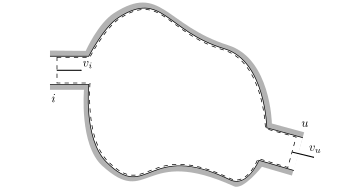
\includegraphics{fig/controlevolumes/Controlevolume_een_in_en_uitstroming}
	\end{frame}
%%%%%%%%%%%%%%%%%%%%%%%%%%%%%%%%%%%%%%%%%%%%%%%%%%%%%%%%%%%%%%%%%%%%%%%%%%%
  	\begin{frame}
		\frametitle{Stationair controlevolume met één in- en uitstroming}
		\begin{textblock}{5}(0,3)
            	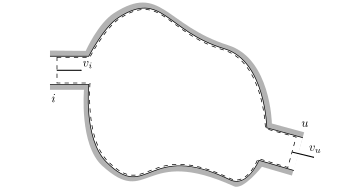
\includegraphics[width=5cm]{fig/controlevolumes/Controlevolume_een_in_en_uitstroming}
        	\end{textblock}
        	\vspace{2cm}
		\begin{equation}
			\rho_i v_{i} A_i = \rho_u v_{u} A_u
			\label{eqn:behoud van massa in een stationair controlevolume met een in en uitstroming}
		\end{equation}
		\pause
		\begin{align}
			F_{x,R} &= p_{u} A_u n_{x,u} + p_{i} A_i n_{x,i} + \dot{m} (v_{x,u}-v_{x,i}) \nonumber \\
			F_{y,R} &= p_{u} A_u n_{y,u} + p_{i} A_i n_{y,i} + \dot{m} (v_{y,u}-v_{y,i}) \\
			F_{z,R} &= p_{u} A_u n_{z,u} + p_{i} A_i n_{z,i} + \dot{m} (v_{z,u}-v_{z,i}) \nonumber
			\label{eqn:behoud van impuls in een stationair controlevolume met een in en uitstroming geprojecteerd2}
		\end{align}
		\pause
		\begin{equation}
			\dot{m} (u_u + \frac{p_u}{\rho_u} + \frac{1}{2}v^2_u + g z_u) - \dot{m} (u_i + \frac{p_i}{\rho_i}+ \frac{1}{2}v^2_i + g z_i) = \dot{Q}-\dot{W}_a
			\label{eqn:behoud van energie in een controlevolume met een in en uitstroming asvermogen}
		\end{equation}
	\end{frame}
%%%%%%%%%%%%%%%%%%%%%%%%%%%%%%%%%%%%%%%%%%%%%%%%%%%%%%%%%%%%%%%%%%%%%%%%%%%
	\begin{frame}
		\frametitle{Toepassing}
		\vspace{1cm}
		\centering
		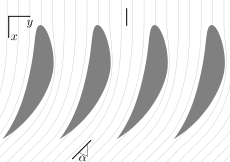
\includegraphics{fig/controlevolumes/Schoepenrij_zonder_controlevolume}
		
		Bepaal de horizontale en verticale kracht op één schoep, veronderstel isotherme stroming zonder warmteoverdracht
	\end{frame}
%%%%%%%%%%%%%%%%%%%%%%%%%%%%%%%%%%%%%%%%%%%%%%%%%%%%%%%%%%%%%%%%%%%%%%%%%%%
\end{document}